No que tange as definições iniciais relacionadas ao \textit{dataset} de casos de Covid-19 em Manaus é importante ressaltar algumas considerações iniciais sobre os dados, levando em consideração que a data de coleta da base de dados para estudo foi no dia 31/07/2020. Sendo assim destaca-se:

\begin{itemize}
    \item Cada exemplo da base de dados é descrito por 36 valores distintos, sendo eles: '\_idade',
    '\_faixa etária', '\_sexo', '\_bairro', '\_classificacao', '\_comorb\_renal', '\_comorb\_diabetes',
    '\_comorb\_imuno', '\_comorb\_cardio', '\_conclusao', '\_dt\_notificacao', '\_taxa',
    '\_dt\_evolucao',
    '\_raca', '\_dt\_sintomas', '\_criterio', '\_tipo\_teste', '\_sintoma\_garganta',
    '\_sintoma\_dispneia',
    '\_sintoma\_febre', '\_sintoma\_tosse', '\_sintoma\_outros', '\_etnia', '\_profiss\_saude',
    '\_srag',
    '\_se\_notificacao', '\_distrito', '\_bairro\_mapa', '\_comorb\_respiratoria',
    '\_comorb\_cromossomica',
    '\_comorb\_hepatica', '\_comorb\_neurologica', '\_comorb\_hemato', '\_comorb\_obessidade',
    '\_origem', '\_evolução'
    \item Segundo a base de dados, em Manaus há cumulativamente 36671 casos confirmados
    \item O período de tempo que a base de dados abrange vai de 01/04/2020 a 31/07/2020
\end{itemize}

Para uma visualização mais concreta e precisa, foi feita uma limpeza na base de dados de casos de COVID-19, entre elas foi feita a remoção das colunas de : \_comorb\_renal', '\_comorb\_diabetes', '\_comorb\_imuno', 
'\_comorb\_cardio', '\_comorb\_respiratoria', '\_comorb\_cromossomica', 
'\_comorb\_hepatica', '\_comorb\_neurologica', '\_comorb\_hemato', '\_comorb\_obessidade', '\_sintoma\_garganta', '\_sintoma\_dispneia', '\_sintoma\_febre', '\_sintoma\_tosse', '\_sintoma\_outros', '\_etnia', '\_raca', '\_profiss\_saude', '\_dt\_evolucao', '\_dt\_sintomas', '\_origem', '\_evolução', '\_criterio'.

\subsubsection{Análise exploratória}
Com a base de dados limpa, pode-se responder alguns questionamentos sobre a estrutura e a disposição dos dados. Apos a limpeza e organização da base de dados é possível se afirmar que do total restaram 36671 exemplos sendo estes descritos por 13 atributos cada, implicando assim em uma queda aproximada de $65\%$ com relação a quantidade original de dados o que leva a concluir que havia uma quantia considerável de dados ruidosos. Sendo assim, a partir desse ponto sempre que for mencionado base de dados essa já corresponde aos dados consistentes filtrados. 

Para se ter uma sensibilidade percentual dentre os casos de COVID-19 dados como recuperados e não recuperados, foi feita uma análise sobre a base de dados obtendo-se o resultado de que $30.72\%$ de todos os casos presentes foram dados como recuperados. Vale ressaltar que a maior quantidade de casos acometidos de COVID-19 foram em mulheres. A Figura ~\ref{fig:uc} demonstra graficamente o resultado.
\begin{figure}[H]
\centering
    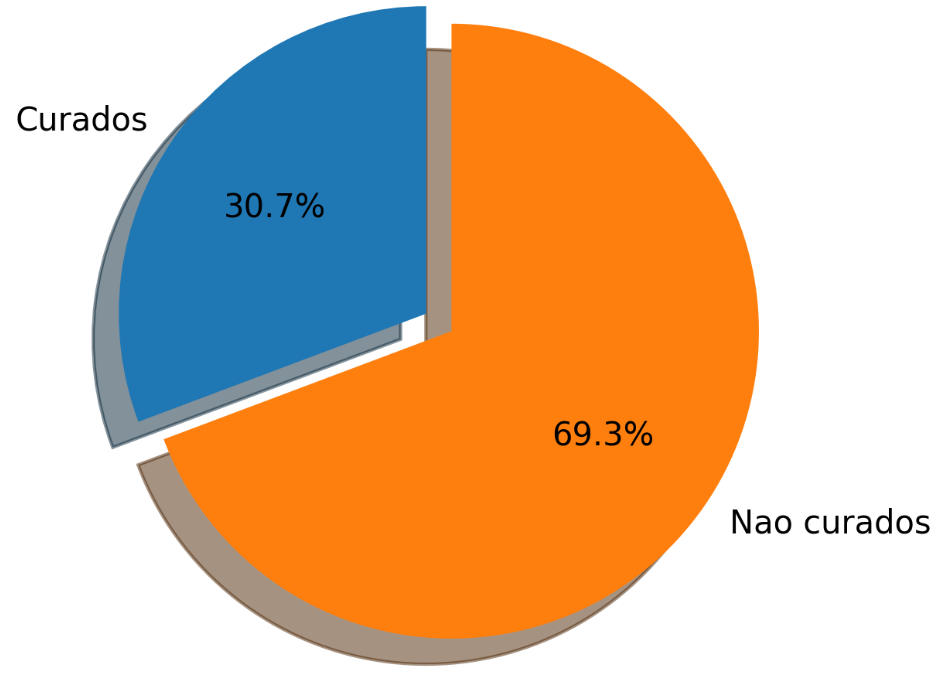
\includegraphics[width=6.5cm]{img/recuperados.png}
    \caption{Gráfico de relação percentual entre recuperados e não recuperados}
    \label{fig:uc} % Toda figura tem que ter um label diferente
\end{figure}

Facilmente percebe-se que não basta um simples calculo percentual para se ter um conhecimento solido sobre os dados, então para um melhor conhecimento sobre a disposição das informações foi feito um estudo estatístico, sobre a idade dos indivíduos que contraíram COVID-19, que envolvem a media e o desvio padrão pois eles permitem ter, respectivamente, uma visão geral da base de dados e também ter uma noção do grau de variação entre o conjunto de dados. Sendo assim, obteve-se o valor de $43.0$ para media que indica que no geral as pessoas que contraíram a doença tem 43 anos e $16.92$ para o desvio padrão que mostra que os valores podem se diferenciar da média por 17 anos indicando um possível intervalo de 26 a 60 anos para os indivíduos que contraíram a doença. Para concluir essa etapa da análise vale ressaltar qual é o verdadeiro intervalo de idade entre os indivíduos listados na base de dados, sendo assim é possível indicar que o individuo mais velho a contrair a doença tinha 120 anos e o mais novo 0 anos (criança recém nascida).

Partindo agora para um estudo que leva mais em consideração a disposição espacial das pessoas que moram em Manaus vale citar que o bairro com maior incidência de casos confirmados foi o bairro CIDADE NOVA com um total de 2008 casos e em contra partida a isso, os 3 bairros com maior quantidade de pessoas dadas como RECUPERADAS foram: CIDADE NOVA, FLORES e CENTRO. Dentre os casos confirmados há ainda aqueles que não fizeram nenhum tipo de exame, no entanto, dentre os que fizeram constata-se que estes foram de 5 tipos diferentes, sendo eles: ECLIA IgG, ELISA IgM, RT-PCR, TESTE RÁPIDO - ANTICORPO, TESTE RÁPIDO - ANTÍGENO. Para se ter uma maior sensibilização sobre os testes feitos tanto de forma quantitativa como percentual observe os gráficos na Figuras~\ref{fig:uc1} e na Figura~\ref{fig:uc2} que mostram a disposição dessas informações.
\begin{figure}[!ht]
\centering
    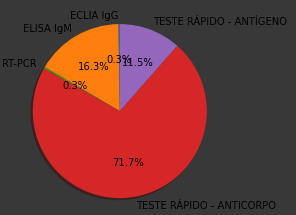
\includegraphics[width=9cm]{img/pizzar.png}
    \caption{Gráfico de percentual de cada teste que foi feito}
    \label{fig:uc1} % Toda figura tem que ter um label diferente
\end{figure}
\begin{figure}[!ht]
\centering
    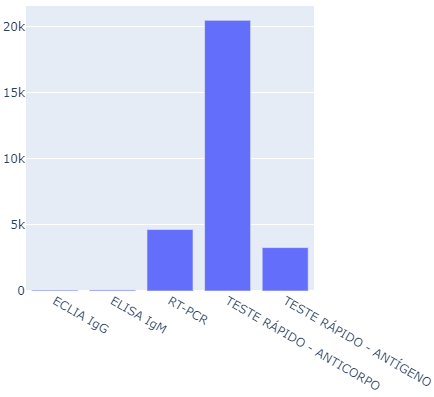
\includegraphics[width=10cm, height=8cm]{img/barrasteste.png}
    \caption{Gráfico de quantidade de cada teste que foi feito}
    \label{fig:uc2} % Toda figura tem que ter um label diferente
\end{figure}

Para finalizar essa etapa de análise exploratória dos dados é importante apontar que a taxa de letalidade foi de 5.5\%, que pode ser confirmado, o que indica um baixo valor percentual. Por fim o coeficiente de correlação de Pearson que visa medir as relações entre variáveis e o que elas representam foi de aproximadamente -0.3309 o que indica um correlação fraca e negativa ou inversa, indicando que as variáveis possuem baixa correlação. Como mostrado na Figura~\ref{fig:normal}, os casos possuem uma distribuição normal.

\begin{figure}[!ht]
\centering
    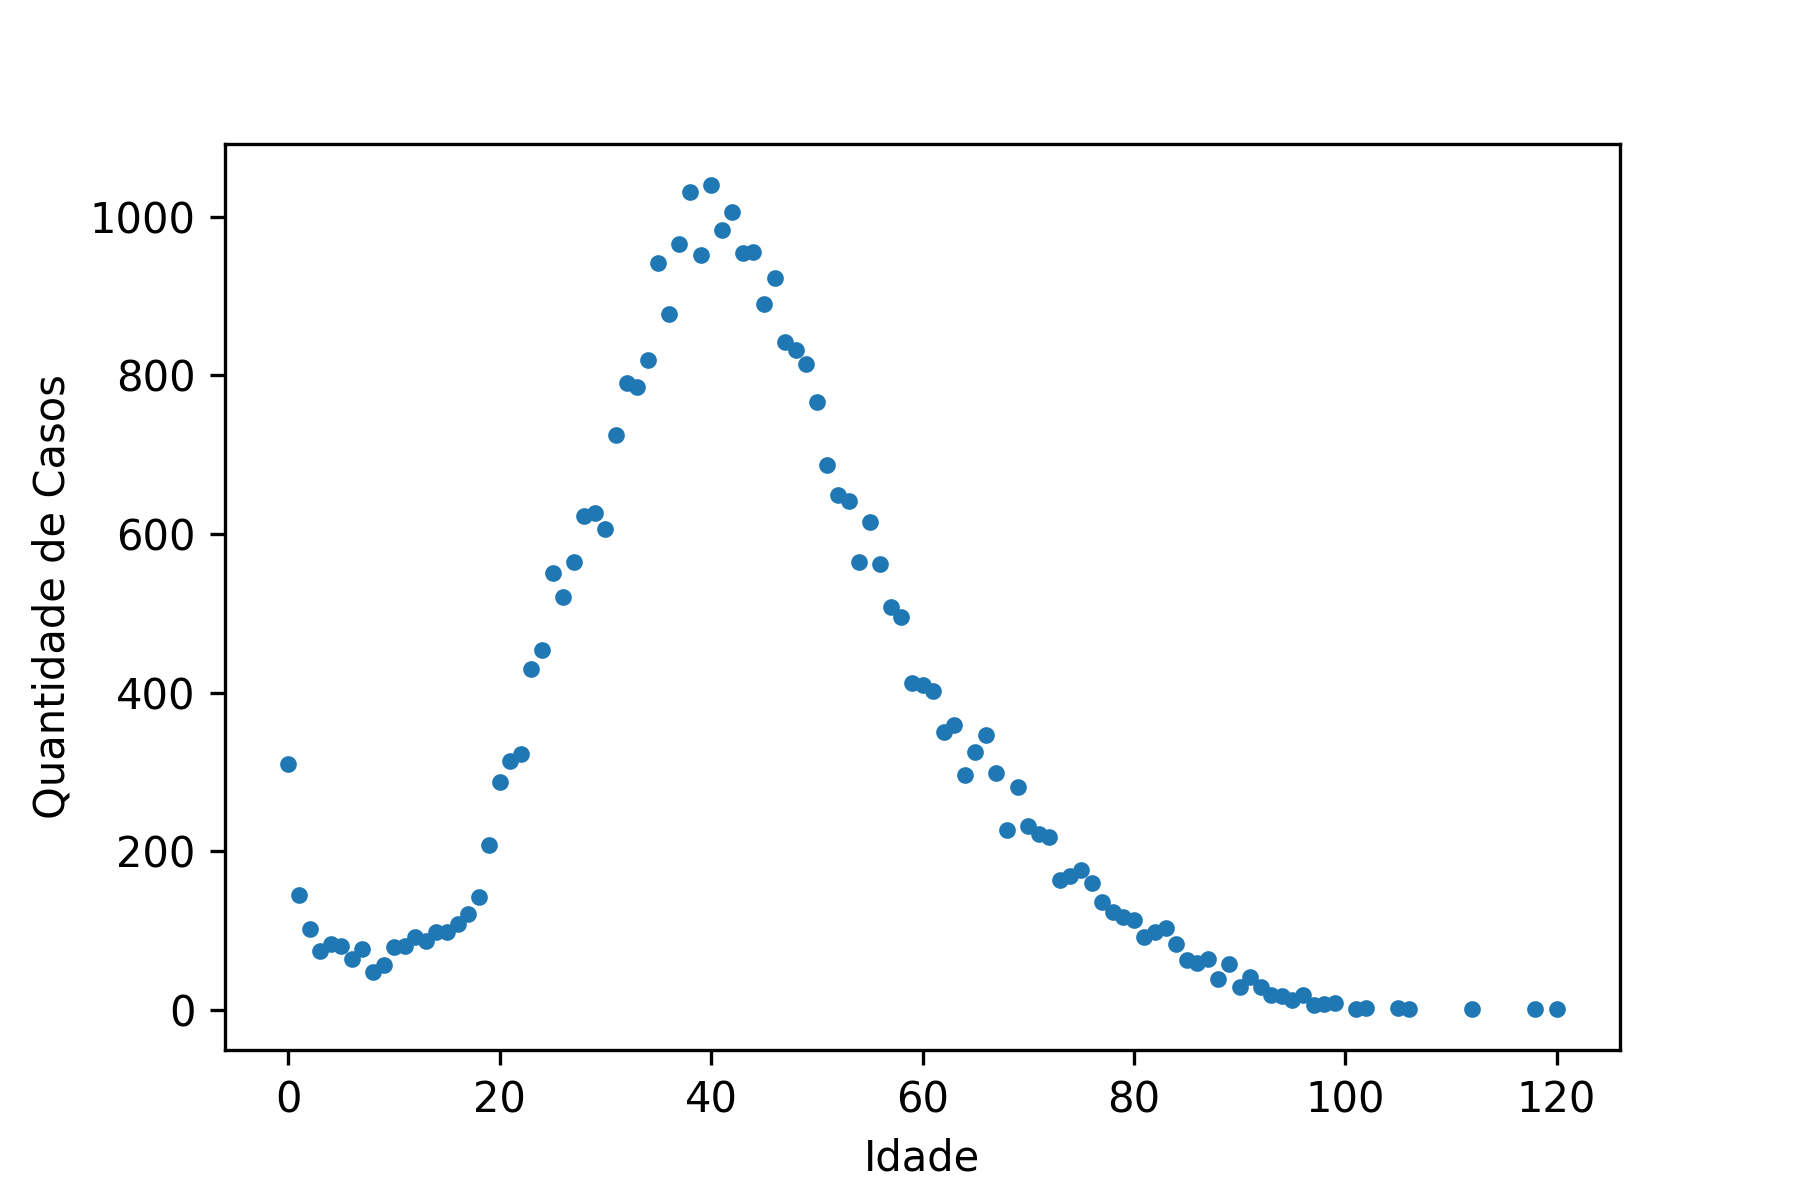
\includegraphics[width=10cm, height=8cm]{img/distribuicaoPorIdade.png}
    \caption{Gráfico de Distribuição por idade}
    \label{fig:normal} % Toda figura tem que ter um label diferente
\end{figure}
